\documentclass[12pt]{zettel}

%\renewcommand{\gregor}{\put(10.0,-3.5){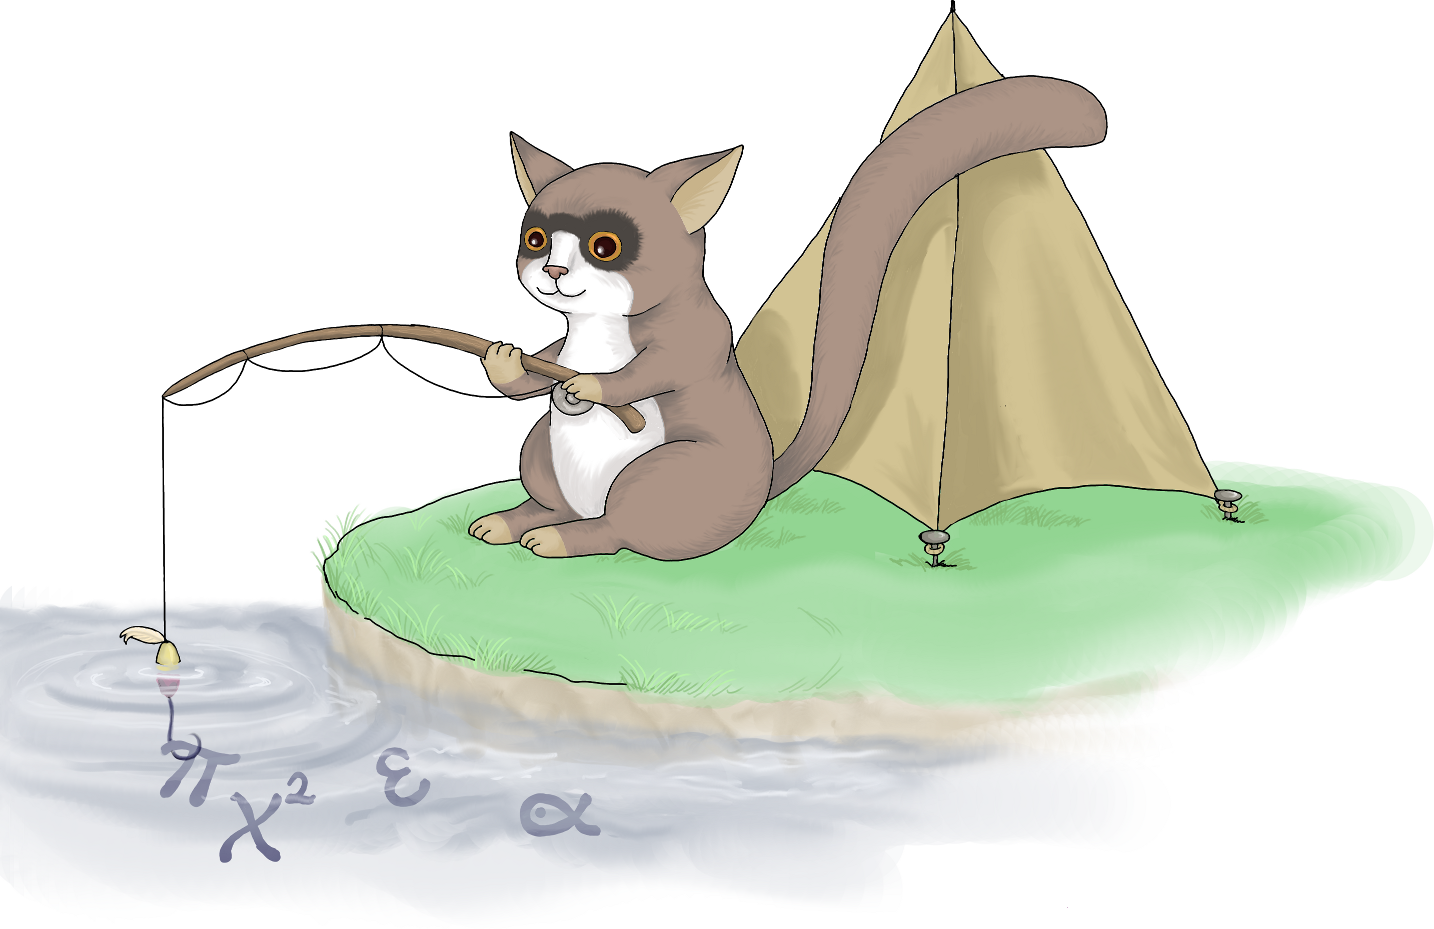
\includegraphics[scale=0.18]{campgregor}}}

\usepackage{framed}
\definecolor{shadecolor}{rgb}{.97,.97,.97}

\geometry{tmargin=1.5cm,bmargin=1.5cm,lmargin=2.5cm,rmargin=2.5cm}

\renewcommand{\gregor}{\put(13.2,-3.0){
\includegraphics[scale=0.18]{cover}}}
\begin{document}

\renewcommand{\betreff}{Mathecamp -- schön war's!}

\makeletterhead{}
\begin{picture}(0,0)
  \put(7.0,-19.0){%
    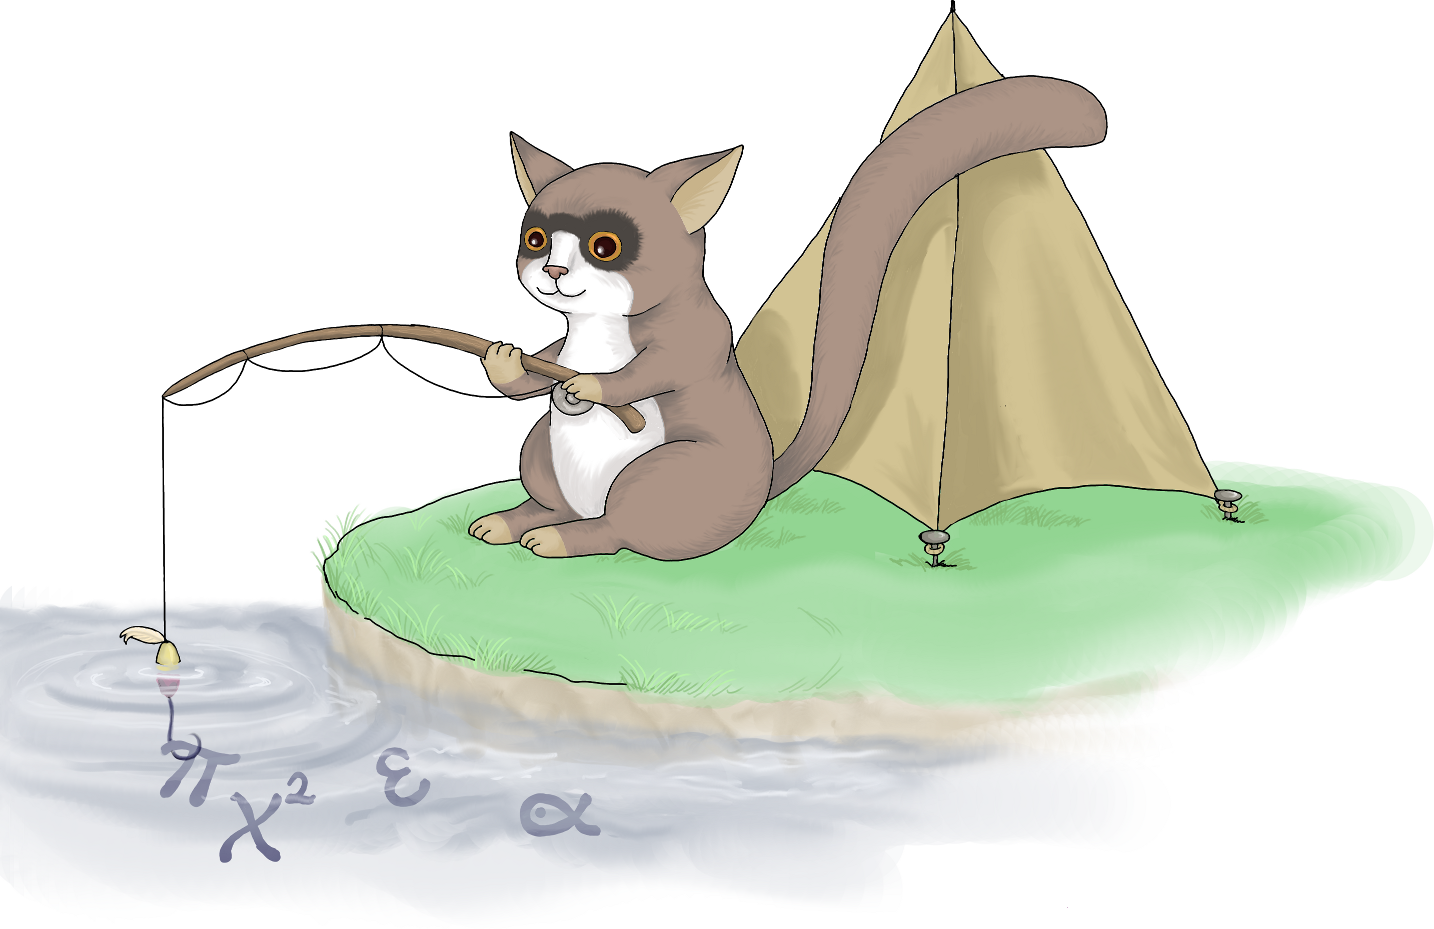
\includegraphics[scale=0.2]{campgregor}
  }
\end{picture}
\vspace{-2em}

Liebe Schülerinnen und Schüler, liebe Eltern,

wir hoffen, dass euch das Mathecamp eine Menge Spaß gemacht habt und ihr auch
viele spannende Themen mitnehmen konntet. Uns Betreuern hat das Camp jedenfalls
viel Freude bereitet.

Nächstes Jahr werden wir das Camp wieder veranstalten -- euren Rückmeldungen
entsprechend dann voraussichtlich sieben statt nur fünf Tage. Diesbezüglich
werden wir euch rechtzeitig informieren.

Wir bedanken uns herzlich bei \emph{Bündnis für Augsburg}, dem
\emph{Mathematisch-Physikalischen Verein} und den Professorinnen und
Professoren der Lehrstühle für \emph{Algebra und Zahlentheorie},
\emph{Angewandte Analysis} und \emph{Nichtlineare Analysis} des Instituts für
Mathematik für ihre Unterstützung.

Besonderer Dank gebührt einem Professor des
Lehrstuhls für \emph{Analysis und Geometrie}, ohne dessen engagierten Einsatz
das Mathecamp nicht denkbar gewesen wäre.

Ferner bedanken wir uns bei Ihnen, liebe Eltern, für die zahlreichen
Spenden.

XXX: Feedback aus der Evaluation inkorporieren; insbesondere von Eltern jetzt
schon mehrmals angesprochene Punkte wie Zimmerzuteilung

XXX: Gruppenfoto und Link zur Fotogalerie

XXX: Sagen, dass wir gerne konstruktive Kritik hören

Euer Mathecamp-Team

{\small Meru Alagalingam, Martin Baur, Ingo Blechschmidt, Tim Dafler, Philipp Düren,
Alexander Engel, Kathrin Helmsauer,
Christian Hübschmann, Jil Hümmer, Sven Prüfer,
Lisa Reischmann, Peter Uebele}

\end{document}
